\chapter{Validación}
\thispagestyle{empty}

\section{Procedimiento}
En este capítulo se mostrarán los procedimientos realizados para validar los requerimientos presentados en la sección \ref{sec:1.5}. Esto incluye:
\begin{itemize}
	\item \textbf{REQ-01:} validar que firmware desarrollado para el equipo maneja correctamente todas las entradas y salidas.
	\item \textbf{REQ-02:} validar que la carga sigue la posición y velocidad indicada por DMX .
	\item \textbf{REQ-03:} validar que el comportamiento del sistema ante el descubrimiento de uno de los 3 errores detectables es la esperada. 
	\item \textbf{REQ-04:} verificar que el funcionamiento del dipswitch es correcto.
\end{itemize}

\section{Procedimiento}
Los requerimientos REQ-01, REQ-02 y REQ-04 se validan simplemente controlando al updown mediante DMX, puesto que de esta manera se utilizan todas las entradas y salidas (que el firmware debe manejar), el sistema de control (que debe asegurar que la carga siga las referencias enviadas por DMX) y el dipswitch (para seleccionar la dirección inicial de DMX).

La prueba se realiza con 9 equipos updown dispuestos en una matriz de 3x3, como se muestra en la figura \ref{fig:4.1}. Todos tienen en su extremo una carga de 3Kg, que es una luminaria cuyas intensidades R, G y B pueden ser controladas mediante 3 canales de DMX.

\begin{figure}[!ht]
	\centering
	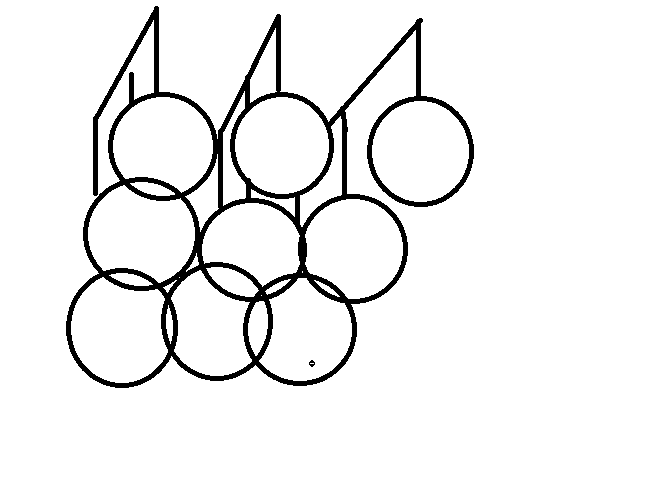
\includegraphics[width=15cm,scale=1]{resources/4_1-matriz3x3updowns.png}
	\caption{Diagrama del sistema motor}
	\label{fig:\thefigure}
\end{figure}

Para controlarlos se utiliza la consola \href{http://www.lighttrader.com/images/HI61020007_L.JPG}{HedgeHog 4}, de HighEnd Systems. 


\textcolor{FIXME}{Explicá: masomenos qué hiciste con la consola, q movimiento configuraste, y poné imágenes comparativas del movimiento en la consola y de los equipos}



Por otro lado, para el requerimiento REQ-01



